%\documentclass[12pt]{report}
%\author{Karthik J, Navya Jose}
%\date{}
%\usepackage{../sem12-lab-record}
\lhead{Date: 19/07/2021}  % For date in header

% REMOVE the % sign in the above lines if you want to
% compile this experiment file separately.

\begin{document}
	
	\chapter{Randomosity of Gamma Emission} % Replace the text with the title of the experiment
	\vspace{-1cm}
	\dateofexp{Date of Experiment: 19/07/2021} 
	% To display date in contents page
	
	\begin{center}% To display date of experiment in the title
		Date of Experiment: 19/07/2021
	\end{center}
	
	%%%%%%%%%%%%%%%%%%%%%%%%%%%%%%%%%%%%%%%%%%%%%
	% THE EXPERIMENT STARTS HERE %
	%%%%%%%%%%%%%%%%%%%%%%%%%%%%%%%%%%%%%%%%%%%%%
	
	\section{Aim}
		To verify that radioactive emission occurs randomly satisfying Poisson distribution when count rate is small but changes to Gaussian distribution as count rate becomes large.
	
	
	\section{Requirements}
	\begin{itemize}
		\item 	GM Counter
		\item 	Gamma Source
	\end{itemize}
	
	\section{Theory}
		The radioactive decay is a random process. Consequently any measurement based on observing the radiation emitted in a nuclear decay is subject to some degree of statistical fluctuations although each measurement for a   radioactive sample is independent of all previous measurements. The deviation of the individual count rates from the average count rate behaves in a predictable manner if we observe a given radioactive nucleus for a time t and define the success as the nuclide decays during the process. then the probability of success p is given by 
		\begin{equation} 
			1-e^{-\lambda t}
		\end{equation}
		where,$\lambda$ is the decay constant. The Poisson	distribution applies when the success probability p very small and the number of counts measured is also very small, say 30.When the average number of success becomes relatively large, say greater than 30, we see that the decay process obeys the Gaussian distribution.
	The latter is described as follows:
	Assume that there is a collection of N independent measurements of the same physical quantity. If each of these N measurements is denoted
	as $x_{1}, x_{2}, . . . , x_{N} ,$the experimental mean is given by
	\begin{equation}
	\bar{x}=\sum\limits_{i=1}^{N}x_i/N
	\end{equation}
	The normal or Gaussian distribution is given by
	\begin{equation}
	p(x)=\frac{1}{\sigma\sqrt{2 \pi }} e^{\frac{-(x-\bar{x})^2}{2 \sigma^2}}
	\end{equation}
	The standard deviation $\sigma^2$=$\bar{x^2}-\bar{x}^2$. 
%	The Poisson distribution is given by
%	\begin{equation}
%	p(x)=\frac{\bar{x}^x e^{-\bar{x}}}{x!}
%	\end{equation}
%	and here, the square of the standard deviation $\sigma^2$=$\bar{x}$
	\section{Procedure}
	
	\begin{enumerate}
		\item 	 Setup the Geiger Mueller Tube and counter. Set the voltage of the GM tube to its optimal operating voltage, which should be around 450 volts.
		\item 	  Don’t put any source in the the lead Castle. Also remove all the sources in the vicinity of the castle. Take three independent readings of the background counts for a pre-set time of 30 seconds.
		\item 	 Place a radioactive beta source far away from the window of GM tube so that approximately 100 counts are recorded in a time period of 30 seconds.
		\item  Set the time for 3000 seconds and note the readings at the end of 30.
	    \item Make class intervals and place each count in its class interval. Find the frequency of occurrence of each class interval.
		\item  	Plot the frequency v/s the average of class interval and join the points by a smooth curve.
        \item Determine the standard deviation of the counts obtained and plot the Gaussian function in equation using the data and the standard deviation. Verify that the nature of the two graphs are same.
		
	\end{enumerate}
	
	\section{Observations \& Graph}
	\begin{equation}
	\bar{x}=3833.18
	\end{equation}
	
	\begin{equation}
	\sigma=49.45032139
	\end{equation}
	
	\begin{longtable}{|r|r|r|r|}
\hline
\multicolumn{1}{|l|}{Counts} & \multicolumn{1}{l|}{Difference} & \multicolumn{1}{l|}{Square} & \multicolumn{1}{l|}{p(x)} \\ \hline
3937                         & 103.9                           & 10795.21                    & 0.0008876250311           \\ \hline
3806                         & -27.1                           & 734.41                      & 0.00694440409             \\ \hline
3806                         & -27.1                           & 734.41                      & 0.00694440409             \\ \hline
3853                         & 19.9                            & 396.01                      & 0.007441922098            \\ \hline
3849                         & 15.9                            & 252.81                      & 0.007663044908            \\ \hline
3949                         & 115.9                           & 13432.81                    & 0.0005176175373           \\ \hline
3859                         & 25.9                            & 670.81                      & 0.007035301349            \\ \hline
3951                         & 117.9                           & 13900.41                    & 0.0004704200292           \\ \hline
3808                         & -25.1                           & 630.01                      & 0.007094238267            \\ \hline
3764                         & -69.1                           & 4774.81                     & 0.003039799174            \\ \hline
3874                         & 40.9                            & 1672.81                     & 0.005731977367            \\ \hline
3784                         & -49.1                           & 2410.81                     & 0.004929122338            \\ \hline
3767                         & -66.1                           & 4369.21                     & 0.003302649081            \\ \hline
3815                         & -18.1                           & 327.61                      & 0.007546734702            \\ \hline
3849                         & 15.9                            & 252.81                      & 0.007663044908            \\ \hline
3893                         & 59.9                            & 3588.01                     & 0.003874659006            \\ \hline
3899                         & 65.9                            & 4342.81                     & 0.003320525101            \\ \hline
3836                         & 2.9                             & 8.41                        & 0.008055717841            \\ \hline
3830                         & -3.1                            & 9.61                        & 0.00805374149             \\ \hline
3774                         & -59.1                           & 3492.81                     & 0.003950820591            \\ \hline
3867                         & 33.9                            & 1149.21                     & 0.00637970328             \\ \hline
3893                         & 59.9                            & 3588.01                     & 0.003874659006            \\ \hline
3828                         & -5.1                            & 26.01                       & 0.00802677991             \\ \hline
3764                         & -69.1                           & 4774.81                     & 0.003039799174            \\ \hline
3830                         & -3.1                            & 9.61                        & 0.00805374149             \\ \hline
3814                         & -19.1                           & 364.81                      & 0.007489549568            \\ \hline
3839                         & 5.9                             & 34.81                       & 0.00801234995             \\ \hline
3772                         & -61.1                           & 3733.21                     & 0.00376131439             \\ \hline
3719                         & -114.1                          & 13018.81                    & 0.0005633424078           \\ \hline
3849                         & 15.9                            & 252.81                      & 0.007663044908            \\ \hline
3778                         & -55.1                           & 3036.01                     & 0.004337619367            \\ \hline
3879                         & 45.9                            & 2106.81                     & 0.005245235486            \\ \hline
3779                         & -54.1                           & 2926.81                     & 0.004435560107            \\ \hline
3840                         & 6.9                             & 47.61                       & 0.007991407213            \\ \hline
3779                         & -54.1                           & 2926.81                     & 0.004435560107            \\ \hline
3827                         & -6.1                            & 37.21                       & 0.008008419011            \\ \hline
3826                         & -7.1                            & 50.41                       & 0.007986833291            \\ \hline
3867                         & 33.9                            & 1149.21                     & 0.00637970328             \\ \hline
3820                         & -13.1                           & 171.61                      & 0.007791336874            \\ \hline
3793                         & -40.1                           & 1608.01                     & 0.005808429844            \\ \hline
3857                         & 23.9                            & 571.21                      & 0.007180046354            \\ \hline
3803                         & -30.1                           & 906.01                      & 0.006704969319            \\ \hline
3821                         & -12.1                           & 146.41                      & 0.007831586668            \\ \hline
3844                         & 10.9                            & 118.81                      & 0.007875908391            \\ \hline
3873                         & 39.9                            & 1592.01                     & 0.005827463451            \\ \hline
3840                         & 6.9                             & 47.61                       & 0.007991407213            \\ \hline
3788                         & -45.1                           & 2034.01                     & 0.005323897396            \\ \hline
3800                         & -33.1                           & 1095.61                     & 0.006450007124            \\ \hline
3869                         & 35.9                            & 1288.81                     & 0.006200174481            \\ \hline
3898                         & 64.9                            & 4212.01                     & 0.003410530132            \\ \hline
\end{longtable}
		The plot of Probability versus count is shown in figure \ref{fig:plot}.\\
		
		The plot of Gaussian Function is shown in figure \ref{fig:plot1}
		
		\begin{figure}
			\centering
			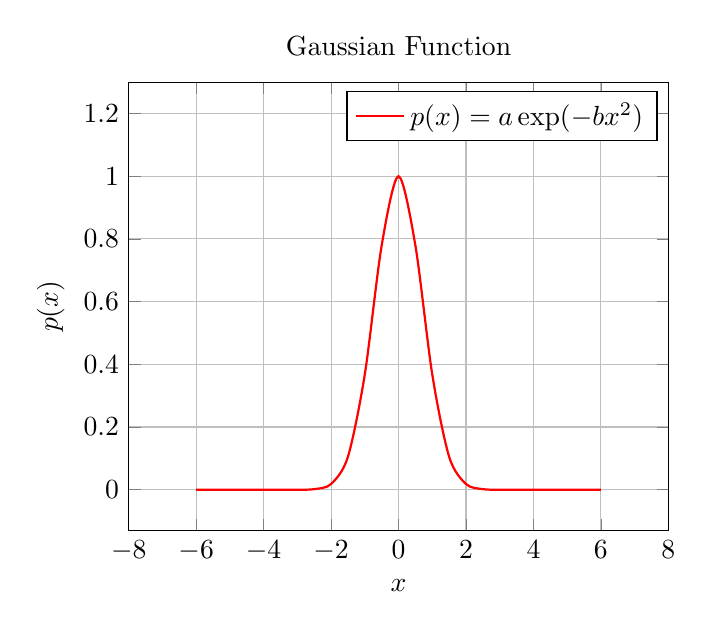
\begin{tikzpicture}
				\begin{axis} [title={Gaussian Function}, grid=major, xlabel = $x$, ylabel = $p(x)$, xmin=-8,xmax=8, ymax=1.3, ytick={-0.2,0,...,1.2}]
					\addplot[color=red, domain=-6:6, thick, smooth] {e^(-x^2)};
					\addlegendentry{$p(x) = a\exp(-bx^2)$}
				\end{axis}
			\end{tikzpicture}
			\caption{}
			\label{fig:plot1}
		\end{figure}

	\section{Result}
Randomosity of radioactive gamma emission is verified first by showing that for small count rates,the decay process satisfies Poisson distribution but for large count rates it follows Gaussian distribution.
	
	%	\section{References}
	
\end{document}